\documentclass[tikz,border=10pt]{standalone}
% Scale s = 0.016842 cm/px (from STYLE METRICS); origin at D
\begin{document}
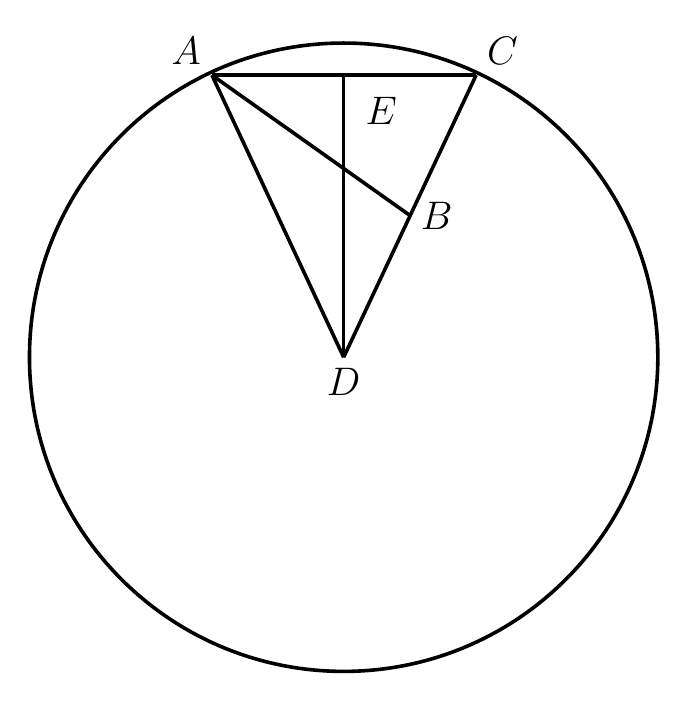
\begin{tikzpicture}[line join=round, line width=1.3pt,
  every node/.style={font=\fontsize{13.5}{16.2}\selectfont}]
  % Points (TikZ units, origin at D)
  \coordinate (D) at (0,0);
  \coordinate (A) at (-1.6725,3.5823);
  \coordinate (C) at (1.6825,3.5823);
  \coordinate (E) at (0,3.5823);
  \coordinate (B) at (0.8421,1.8005);
  % Circle centred at D, radius slightly enlarged (~1%) to match original extent
  \draw (D) circle (3.99);
  % Chord AC (passes through E)
  \draw (A) -- (C);
  % Vertical ED
  \draw (E) -- (D);
  % Segment AB
  \draw (A) -- (B);
  % Radii DA and DC (B lies on DC)
  \draw (D) -- (A);
  \draw (D) -- (C);
  % Labels
  \node[above left] at (A) {$A$};
  \node[above right] at (C) {$C$};
  % E label moved below-right of vertex E, clear of chord AC
  \node[below right=4pt] at (E) {$E$};
  \node[right] at (B) {$B$};
  \node[below] at (D) {$D$};
\end{tikzpicture}
\end{document}